\chapter{Testiranje detekcije i \mbox{automatske} reakcije}

Cilj je ovog poglavlja funkcionalno provjeriti dvije sposobnosti sustava koje nisu obuhvaćene usporedbom podsustava za pohranu iz prethodnog poglavlja.
Sposobnost prepoznavanja sumnjivog ponašanja u prometu te sposobnost automatskog odgovora na prepoznatu prijetnju. Provjera se provodi kao niz
nadziranih testova u kojima se s poznatog klijenta izaziva određeni obrazac prometa, a potom se promatra cijeli lanac od Zeekova upozorenja u
\texttt{notice.log}, preko skripte \texttt{auto\_reaction.py}, do izmjene elemenata skupa \texttt{denylist} u tablici \texttt{diplomski}. Svaki se test
prati po izvorišnoj adresi, čime se uspostavlja jednoznačna veza između izazvanog događaja, zabilježenog upozorenja i poduzete reakcije. Navode se
isključivo stvarno izmjereni zapisi.

\section{Testno okruženje i metodologija}

Testovi su provedeni na sklopovlju opisanom u poglavlju arhitekture. Prijenosno računalo istovremeno obavlja uloge usmjernika i bežične pristupne točke, pri
čemu je sučelje \texttt{enp2s0} povezano prema vanjskoj mreži (eduroam), a sučelje \texttt{wlan1} podiže pristupnu točku za lokalnu podmrežu
\texttt{10.0.1.0/24}. Postavljene su dvije jasno razdvojene uloge:

\begin{itemize}
\item \textbf{Napadač} --- klijent priključen na pristupnu točku. U svim je
testovima detekcije korišten mobilni uređaj s adresom \texttt{10.0.1.94}.
\item \textbf{Branitelj i senzor} --- samo prijenosno računalo
(\texttt{10.0.1.1}), na kojem rade Zeek, \texttt{nftables} i skripta
\texttt{auto\_reaction.py}.
\end{itemize}

Zeek promet hvata na sučelju \texttt{wlan1}, dakle prije prevođenja mrežnih adresa, pa izvorišne adrese ostaju stvarne adrese uređaja u lokalnoj mreži - ta
je činjenica ključna jer omogućuje pripisivanje upozorenja pojedinom uređaju. 

Za izazivanje pojedinih obrazaca prometa korišteni su sljedeći alati: \texttt{nmap} za skeniranje portova, \texttt{sshpass} za automatske ponavljane pokušaje
prijave putem \texttt{SSH}, \texttt{curl} za uspostavljanje veze alatom prema adresi iz datoteke \texttt{intel.dat} za podudaranje
s indikatorom kompromitacije te \texttt{hping3} za lažiranje izvorišne adrese pri ispitivanju ograničenja.

Reakcija se temelji na sljedećem ponašanju skripte: po prepoznavanju obavijesti izvorišna adresa (\texttt{src}) dodaje se kao element skupa \texttt{denylist} s
vremenskim ograničenjem od 30 sekundi, osim ako se nalazi na popisu dopuštenih adresa. U redovnom radu popis dopuštenih adresa sadrži \texttt{127.0.0.1} i
\texttt{10.0.1.1}; adresa \texttt{10.0.1.94} dodana je na taj popis isključivo za potrebe testiranja.

Radi provjere lažno pozitivnih odziva kroz pristupnu je točku propušten uobičajen promet (pregledavanje weba, dohvaćanje datoteka, ažuriranja sustava) 
tijekom 3 sata 38 minuta 41 sekunde. Nijedan obrazac nije premašio pragove definirane u \texttt{local.zeek} (50 različitih portova u pet minuta odnosno 
15 SSH veza), pa skup \texttt{denylist} nije popunjen niti je jedan legitiman uređaj blokiran.
\section{Provjera toka podataka}

Prije ispitivanja detekcije potvrđuje se da podatci prolaze cijelim lancem obrade. Na klijentu se uspostavi veza, nakon čega se utvrđuje da je nastao
zapis u \texttt{conn.log}, da ga je preuzeo agent (Telegraf odnosno Filebeat), da je pohranjen u pripadnoj bazi te da je vidljiv na odgovarajućem prikazu u
Grafani. Na nadzornoj ploči, na slici \ref{fig:dashboard-start}, izravno se očitava da podatci pristižu - prikazani su broj veza u minuti, raspodjela protokola
te ljestvice najčešćih izvorišnih i odredišnih adresa, u kojima se pojavljuju stvarne adrese klijenata iz lokalne podmreže. Time je potvrđeno da je tok
podataka cjelovit i da se izvorišne adrese očuvane na sučelju \texttt{wlan1} ispravno prenose do prikaza.

\begin{figure}[h]
    \centering
    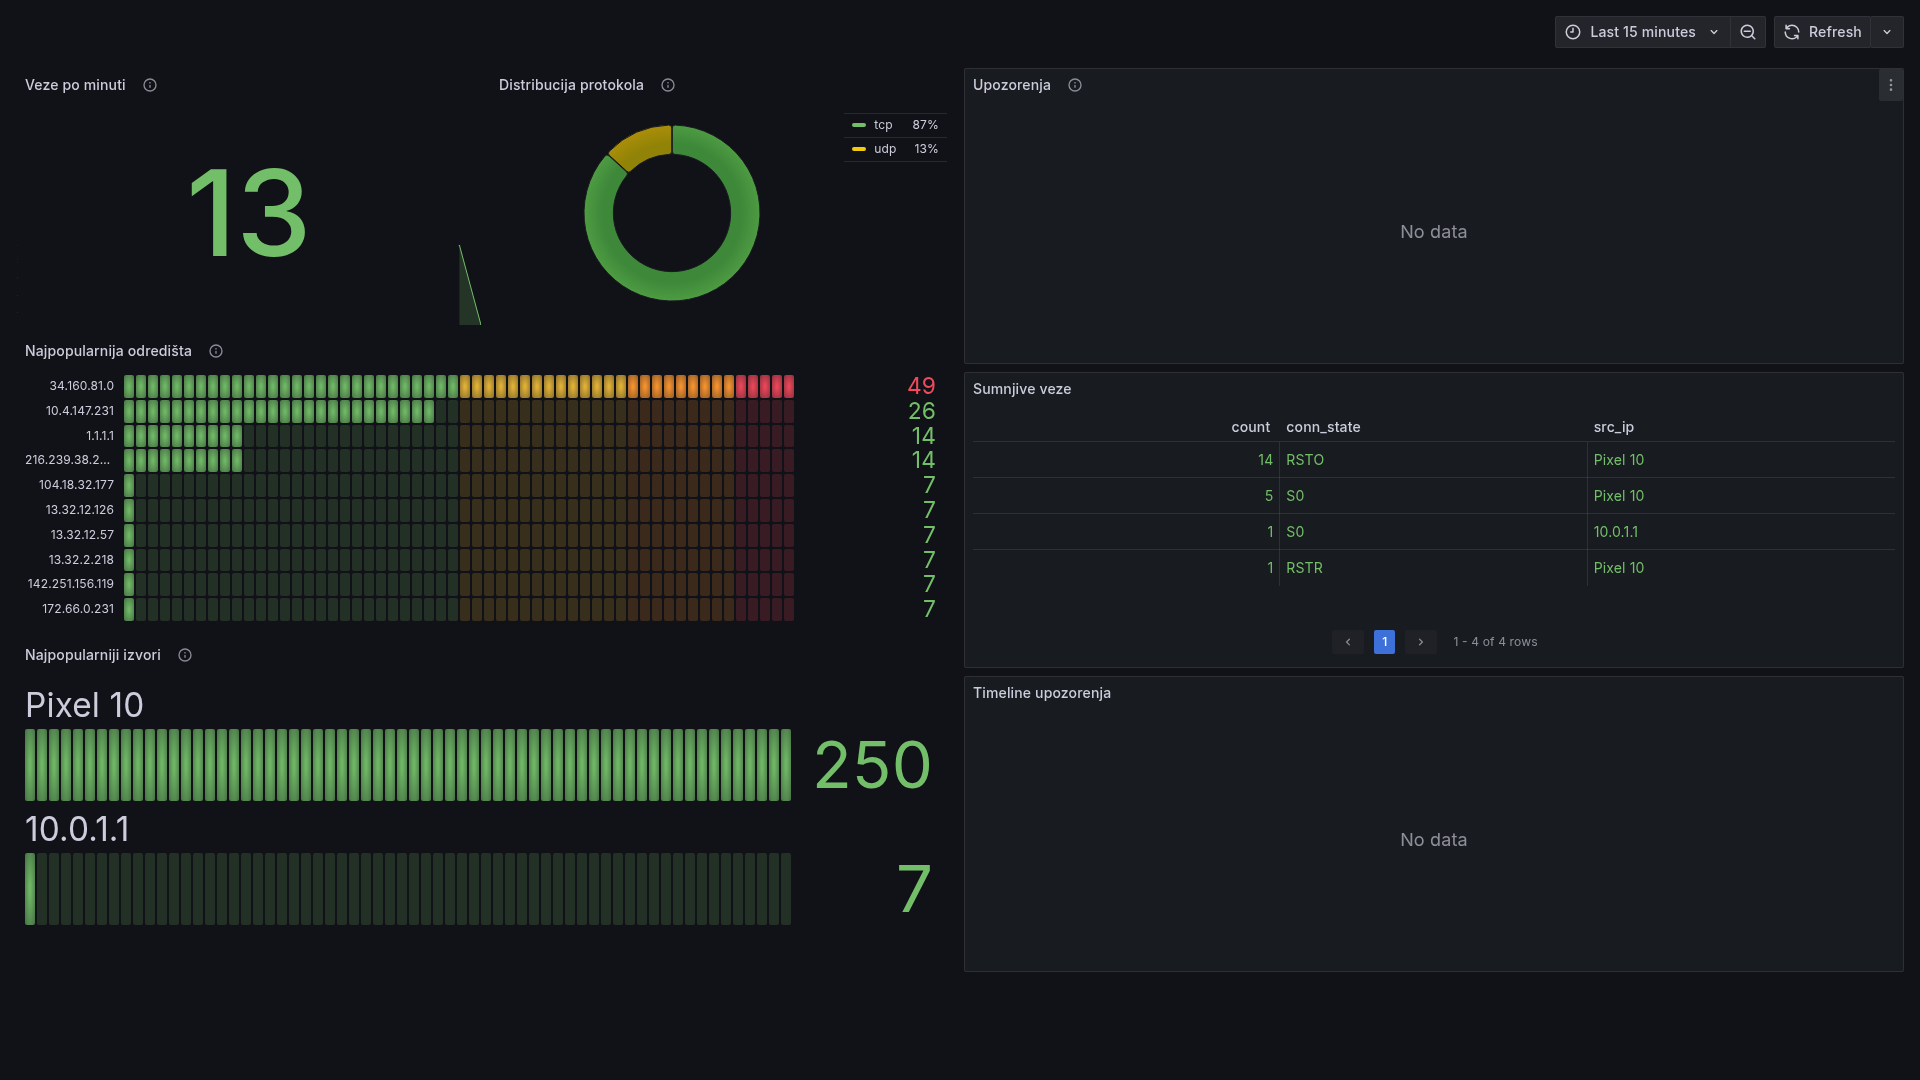
\includegraphics[width=\linewidth]{slike/dashboard_start.png}
    \caption{Prikaz podataka na nadzornoj ploči: broj veza u minuti, raspodjela
    protokola te najčešći izvori i odredišta; u promatranom razdoblju nema
    upozorenja (osnovno stanje prometa)}
    \label{fig:dashboard-start}
\end{figure}

\section{Testiranje detekcije}

Provedena su tri testa detekcije: skeniranje portova, bruteforce SSH prijave i podudaranje s indikatorom kompromitacije. Svi su izvedeni s klijenta
\texttt{10.0.1.94}, osim lažiranog skeniranja iz odjeljka o ograničenjima. Sva tri tipa upozorenja vidljiva su na vremenskoj crti nadzorne ploče
na slici \ref{fig:timeline}, s pripadnim izvorišnim adresama.

\begin{figure}[h]
    \centering
    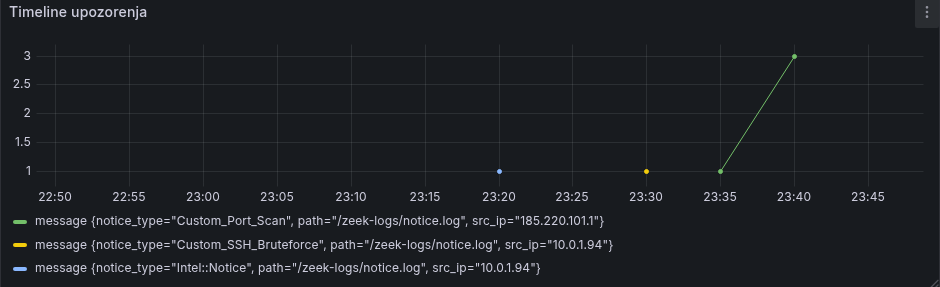
\includegraphics[width=\linewidth]{slike/timeline_upozorenja.png}
    \caption{Vremenska crta upozorenja: \texttt{Custom\_Port\_Scan}
    (\texttt{185.220.101.1}) te \texttt{Custom\_SSH\_Bruteforce} i
    \texttt{Intel::Notice} (oba \texttt{10.0.1.94})}
    \label{fig:timeline}
\end{figure}

\subsection{Skeniranje portova}

Skeniranje je izazvano s klijenta \texttt{10.0.1.94} naredbom \texttt{nmap -Pn -T4 10.0.1.1}. Prekoračenjem praga od 50 različitih
kontaktiranih portova prema istom cilju, Zeek je zabilježio upozorenje tipa \texttt{Custom\_Port\_Scan} sa stvarnom izvorišnom adresom
\texttt{10.0.1.94} u ispisu \ref{lst:notice-portscan}. Detektor djeluje na događaju \texttt{new\_connection}, pa reagira na pokušaj veze i ne ovisi o
njezinom uspješnom uspostavljanju.

\begin{lstlisting}[caption={Upozorenje o skeniranju portova (\texttt{notice.log})}, label={lst:notice-portscan}]
    {"ts":1781467564.943518,"note":"Custom_Port_Scan",
    "msg":"Moguci port scan: 10.0.1.94 kontaktirao 50 razlicitih portova na 10.0.1.1",
    "src":"10.0.1.94","actions":["Notice::ACTION_LOG"],
    "email_dest":[],"suppress_for":30.0}
\end{lstlisting}

\subsection{Bruteforce SSH prijave}

Bruteforce je izveden s klijenta \texttt{10.0.1.94} kao 40 uzastopnih neuspjelih pokušaja prijave putem \texttt{SSH} (alat \texttt{sshpass}) prema
domaćinu. Korišteni prilagođeni detektor broji \emph{učestalost veza} prema portu 22, neovisno o ishodu autentikacije, te je komplementaran Zeekovu
detektoru \texttt{SSH::Password\_Guessing} koji radi na temelju zaključene autentikacije. Pri pragu od 15 veza zabilježeno je upozorenje tipa
\texttt{Custom\_SSH\_Bruteforce}; tijekom 40 pokušaja istek prozora suzbijanja (30 s) doveo je do druge obavijesti pri 36 veza \ref{lst:notice-ssh}.

\begin{lstlisting}[caption={Dvije obavijesti o SSH bruteforceu tijekom istog niza pokušaja (\texttt{notice.log})}, label={lst:notice-ssh}]
    {"ts":1781468972.322033,"note":"Custom_SSH_Bruteforce",
    "msg":"Moguci SSH bruteforce: 10.0.1.94 otvorio 15 konekcija prema portu 22 na 10.0.1.1",
    "src":"10.0.1.94","suppress_for":30.0}
    {"ts":1781469003.721936,"note":"Custom_SSH_Bruteforce",
    "msg":"Moguci SSH bruteforce: 10.0.1.94 otvorio 36 konekcija prema portu 22 na 10.0.1.1",
    "src":"10.0.1.94","suppress_for":30.0}
\end{lstlisting}

Obavijesti su vidljive i na nadzornoj ploči, na slici \ref{fig:ssh-grafana}, gdje je za izvor \texttt{10.0.1.94} zabilježeno više detekcija
\texttt{Custom\_SSH\_Bruteforce} pri pragovima od 15 te 35-36 veza.

\begin{figure}[h]
    \centering
    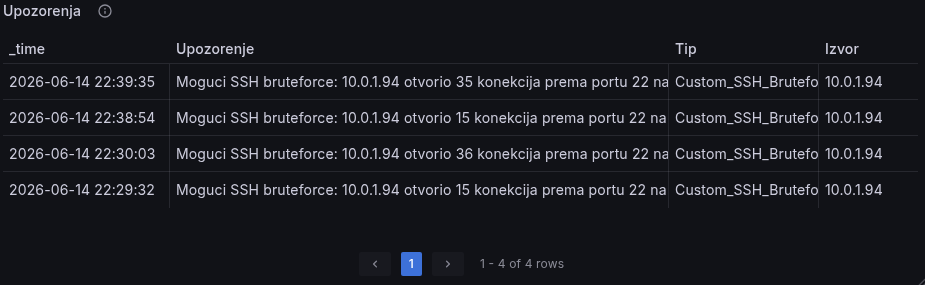
\includegraphics[width=\linewidth]{slike/ssh_bruteforce_grafana.png}
    \caption{Upozorenja o SSH bruteforceu na nadzornoj ploči (izvor
    \texttt{10.0.1.94})}
    \label{fig:ssh-grafana}
\end{figure}

\subsection{Podudaranje s indikatorom kompromitacije}

Podudaranje je izazvano uspostavljanjem veze s klijenta \texttt{10.0.1.94} prema adresi unaprijed unesenoj u datoteku \texttt{intel.dat}. Putem okvira
\engl{Intel framework} (skripte \texttt{intel/seen} i \texttt{intel/do\_notice}) Zeek poklapa adrese na događaju uspostavljene veze
(\texttt{connection\_established}); za test je stoga ključno da se veza \emph{uspostavi}, neovisno o ishodu na aplikacijskoj razini. Veza je rezultirala
neuspjehom pri \engl{TLS} pregovaranju, ali je TCP rukovanje dovršeno, što je dovoljno za poklapanje. Zeek je zabilježio upozorenje tipa
\texttt{Intel::Notice} u ispisu \ref{lst:notice-ioc}.

\begin{lstlisting}[caption={Upozorenje o podudaranju s indikatorom kompromitacije (\texttt{notice.log})}, label={lst:notice-ioc}]
    {"ts":1781471801.228362,"id.orig_h":"10.0.1.94","id.resp_h":"172.66.147.243",
    "id.resp_p":443,"proto":"tcp","note":"Intel::Notice",
    "msg":"Intel hit on 172.66.147.243 at Conn::IN_RESP",
    "src":"10.0.1.94","dst":"172.66.147.243","p":443,"suppress_for":3600.0}
\end{lstlisting}

Za testni je indikator korištena dostupna javna adresa, što je uobičajena i sigurna praksa pri provjeri Intel okvira. Vrijednost \texttt{suppress\_for}
ovdje iznosi 3600 sekundi (zadani interval suzbijanja obavijesti); taj se interval prema potrebi snižava postavkom u \texttt{local.zeek}, čime se trguje
između količine obavijesti i odzivnosti te je on odvojen od \texttt{TIMEOUT} kojeg se postavlja za duljinu trajanja blokade unutar nft skupa \texttt{denylist}
u tablici \texttt{diplomski}.

\section{Testiranje automatske reakcije}

\subsection{Blokiranje izvora i istek blokade}

Reakcija je promatrana na primjeru skeniranja portova iz ispisa \ref{lst:notice-portscan}. Prije testa skup \texttt{denylist} bio je
prazan; ubrzo nakon detekcije izvorišna se adresa nalazi u skupu, uz preostalo vrijeme do isteka koje očitava jezgra u ispisu \ref{lst:nft-block}. Skripta
\texttt{auto\_reaction.py} pritom je ispisala odgovarajuću potvrdu u ispisu \ref{lst:reaction-portscan}.

\begin{lstlisting}[language=bash, caption={Skup \texttt{denylist} prije i tijekom blokade}, label={lst:nft-block}]
    # prije:
    table ip diplomski {
            set denylist { type ipv4_addr ; timeout 30s }
    }
    # tijekom blokade:
    table ip diplomski {
            set denylist {
                    type ipv4_addr
                    timeout 30s
                    elements = { 10.0.1.94 expires 22s818ms }
            }
    }
\end{lstlisting}

\begin{lstlisting}[caption={Ispis skripte \texttt{auto\_reaction.py}},
    label={lst:reaction-portscan}]
    [!] Detektiran Custom_Port_Scan.
    [!] Blokiran IP: 10.0.1.94
    [+] Istekla evidencija blokade: 10.0.1.94
\end{lstlisting}

Trajanje blokade određeno je vremenskim ograničenjem skupa (\texttt{timeout 30s}). Nakon isteka
blokade jezgra automatski uklanja element, bez intervencije skripte ili operatora. To je moguće potvrditi porukom o isteku u svakom testu te ponovnim pregledom praznog skupa.

Za odlaznu vezu prema indikatoru kompromitacije skripta blokira polje \texttt{src} iz obavijesti, a to je \emph{unutarnji} klijent koji je ostvario
vezu (\texttt{10.0.1.94}), a ne vanjska maliciozna adresa. Riječ je o namjernom postupku. Vanjska je adresa izvan dosega upravljanja, dok se
blokiranjem unutarnjeg domaćina ograničava daljnja komunikacija potencijalno kompromitiranog uređaja.

Blokada je potvrđena i pregledom skupa nakon podudaranja s indikatorom kompromitacije. U skupu \texttt{denylist} nalazi se unutarnji klijent
\texttt{10.0.1.94}, a ne vanjska adresa indikatora što je vidljivo u ispisu \ref{lst:nft-ioc}.

\begin{lstlisting}[language=bash, caption={Skup \texttt{denylist} nakon podudaranja s indikatorom kompromitacije},label={lst:nft-ioc}]
    table ip diplomski {
            set denylist {
                    type ipv4_addr
                    timeout 30s
                    elements = { 10.0.1.94 expires 11s813ms }
            }
}
\end{lstlisting}

\subsection{Zaštita vlastite infrastrukture popisom dopuštenih adresa}

Provjereno je da skripta ne reagira kad je izvorišna adresa na popisu dopuštenih. U testu je adresa \texttt{10.0.1.94} privremeno dodana na popis,
nakon čega je ponovljen SSH bruteforce. Zeek je i dalje zabilježio upozorenje \texttt{Custom\_SSH\_Bruteforce} (detekcija nije izostala), no skup
\texttt{denylist} ostao je prazan, a skripta nije poduzela reakciju, što je vidljivo u ispisu \ref{lst:whitelist}. Time je potvrđeno da popis dopuštenih adresa
sprječava blokiranje povjerljivih izvora bez utjecaja na detekciju.

\begin{lstlisting}[caption={Detekcija bez reakcije za adresu na popisu dopuštenih}, label={lst:whitelist}]
    # WHITELIST = {"127.0.0.1", "10.0.1.1", "10.0.1.94"}
    [*] Nadzor pokrenut nad zeek-logs/notice.log
    # upozorenje se nalazi u notice.log, ali skripta nije reagirala
    # skup denylist ostao prazan
    # sustav radi kako bi i trebao
\end{lstlisting}

\section{Ograničenja uočena testiranjem}

\subsection{Lažiranje izvorišne adrese}

Reakcija se temelji na izvorišnoj adresi iz obavijesti, pa je njezina ispravnost ograničena ispravnošću te adrese. Ograničenje je provjereno
namjernim lažiranjem izvorišne adrese alatom \texttt{hping3}, kojim je izvedeno skeniranje portova uz krivotvorenu adresu \texttt{185.220.101.1}
(\texttt{hping3 -S -{}-spoof 185.220.101.1 -{}-scan 1-1000 10.0.1.94}). Zeek je zabilježio upozorenje s krivotvorenom adresom, a skripta je upravo nju dodala u
skup \texttt{denylist} u ispisu \ref{lst:spoof}.

\begin{lstlisting}[language=bash, caption={Ispis denylist}, label={lst:spoof}]
    # notice.log:  "note":"Custom_Port_Scan", "src":"185.220.101.1"
    table ip diplomski {
            set denylist {
                    type ipv4_addr
                    timeout 30s
                    elements = { 185.220.101.1 expires 19s395ms }
            }
    }
\end{lstlisting}

Potvrđeno je očekivano, ali nepoželjno ponašanje. Sustav blokira adresu navedenu u obavijesti, koja ne mora odgovarati stvarnom napadaču. Stvarni
napadač ostaje neblokiran, a lažira li adresu legitimnog uređaja koji nije na popisu dopuštenih, sustav će blokirati taj uređaj. Popis dopuštenih adresa
tu ne pomaže jer štiti samo usmjernik i lokalnog domaćina, a ne i proizvoljne uređaje od povjerenja; štoviše, oslanja se na izvorišnu adresu koja je i sama
krivotvorljiva. Djelotvorno ublažavanje je filtriranje na ulazu sučelja \texttt{wlan1} (odbacivanje paketa čija izvorišna adresa nije iz
\texttt{10.0.1.0/24}), čime se krivotvoreni paket odbacuje prije detekcije.

Valja razlučiti i opseg sposobnosti. Detekcija i reakcija djeluju nad prometom koji Zeek vidi na sučelju \texttt{wlan1}; nepozvani dolazni promet iz širega
područja mreže na sučelju \texttt{enp2s0} odbacuje se zadanom politikom vatrozida \texttt{ufw} i nije zadaća ovoga sloja.

\subsection{Otpornost na nasilni prekid skripte}

Budući da trajanje blokade nameće vremensko ograničenje skupa, a ne sama skripta, nasilni prekid skripte ne ostavlja zaostala vatrozidna pravila.
Prekine li se skripta, elementi skupa svejedno isteknu djelovanjem jezgre, što je u svakom testu potvrđeno automatskim isticanjem blokade. Time se izbjegava
slabost izvedbi u kojima prekid posrednika ostavlja mrežu u nedefiniranom stanju. Podrobnije obrazloženje dano je u poglavlju implementacije.

\subsection{Izloženost nadzornih servisa}

Tijekom skeniranja uočeno je da je na domaćinu \texttt{10.0.1.1} otvoren port \texttt{8086} (InfluxDB), dohvatljiv iz nadziranog segmenta. Nadzorni servisi
(InfluxDB, Grafana) time čine dio površine napada vidljive klijentima, pa bi ih u stvarnoj primjeni trebalo izolirati od nadziranog segmenta. U radu je to kratko
popravljeno ovom linijom u \texttt{docker-compose.yml}: \texttt{"127.0.0.1:8086:8086"} za InfluxDB odnosno \texttt{"127.0.0.1:3000:3000"} za Grafanu.
Svi načini testiranja i mjerenja se mogu naći u dodatku \texttt{benchmark.sh}.